\documentclass[a4paper, 12pt]{article}
\usepackage[utf8]{inputenc} 
\usepackage[english]{babel}
\usepackage[T1]{fontenc}
\usepackage{array,multirow,makecell}
\usepackage{graphicx}
\usepackage{fancyhdr}
\usepackage{booktabs}
\usepackage{wrapfig}
\usepackage{hyperref}
\pagestyle{fancy}
\usepackage{amsmath,amsfonts,amssymb, empheq}
\setcellgapes{1pt}
\usepackage[affil-it]{authblk}
\makegapedcells
\newcolumntype{R}[1]{>{\raggedleft\arraybackslash }b{#1}}
\newcolumntype{L}[1]{>{\raggedright\arraybackslash }b{#1}}
\newcolumntype{C}[1]{>{\centering\arraybackslash }b{#1}} 

%\setcellgapes{1pt}
\makegapedcells

\begin{document}

	\begin{titlepage}
		
		\centering
%\vspace*{0.5cm}
\textsc{{\LARGE \textbf{Université Paris-Est Créteil}}} \\
\vspace*{0.5cm}
\textsc{{\LARGE \textbf{Faculté de Sciences Économiques et de Gestion}}}
\vspace*{1cm}

\begin{center}
	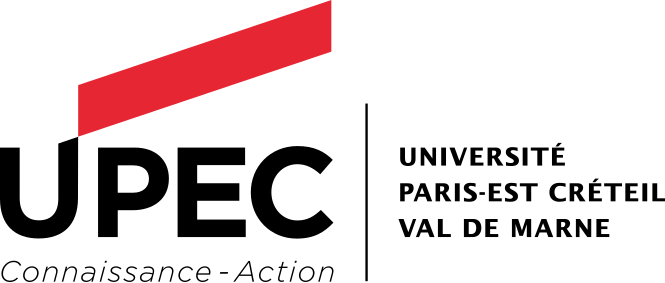
\includegraphics[scale=0.25]{../../UPEC-logo.svg}
\end{center}
\vspace*{1cm}

\LARGE

\textbf{Forecasting with High-Frequency Data:}\\
\textit{An Application of GARCH Models to Stock Market Indices}\\
\vspace{1cm}		
\Large

\vspace{0cm}

\textbf{Issa KACHAOU}\\
\large
\textbf{Thesis advisor : Pierre DURAND} \\
\begin{abstract}
	\noindent
	Financial markets exhibit complex dynamics, making accurate forecasting a critical yet challenging task for investors, analysts, and policymakers. Time series models, such as the Autoregressive Moving Average (ARMA) and the Autoregressive Conditional Heteroskedasticity (ARCH) models, have been widely employed to capture the underlying patterns in financial data. While ARMA models focus on modeling the linear dependence in time series, ARCH models account for the volatility clustering phenomenon often observed in financial markets.
\end{abstract}


\vfill

\Large

\textbf{\today}
		
	\end{titlepage}

\pagestyle{plain}
\part{Introduction}


\part{Methods}

\section{The GARCH model, Bollerslev (1986)}

\[ \sigma_t^2=\alpha_0+\sum_{i=1}^{q}\alpha_i\epsilon_{t-i}^2+\sum_{j=1}^{p}\beta_j\sigma_{t-j}^2=\alpha_0+\alpha(L)\epsilon_t^2+\beta(L)\sigma_t^2\] 
Where 
\[ \alpha_0>0 \; , \; \alpha_i \ge 0 \; , \; \beta_j \ge 0 \; ,\; \forall i, \forall j\]


\part{Results}


\part{Discussion}



\part{Conclusion}

\end{document}